% Chapter 2

\chapter{Learning Bayesian Networks} % Main chapter title

\label{Chapter2} % For referencing the chapter elsewhere, use \ref{Chapter1} 

\lhead{Chapter 2. \emph{Learning}} % This is for the header on each page - perhaps a shortened title
Bayesian networks are directed acyclic graphs (DAG). They are representations of the dependence structure among a set of random variables. The conditional dependencies between the random variables are visualized by directed edges and the random variables themselves are the nodes of the network. Through the directed edges it is possibly to identify a hierarchy. Nodes having edges leading to another node are called parents of the receiving node. Similarly, the receiving node is a child of the source node. Besides the dependence structure the nodes in a Bayesian Network carry a probability distribution conditional on their parents. In the case of discrete distributions this becomes a probability table.\\
The advantage of using a Bayesian Network is that it represents the joint probability over all the random variables considered, so that it is possible to answer conditional queries through the laws of probability theory. Through the structure of the network the joint probability distribution factorizes, leading to less parameters to estimate and a more efficient computation.\\
For the task of the evaluation of natural hazard Bayesian Networks provide a consistent and efficient way to compute the full distribution of the target variable and thus to deal with the associated uncertainties.
\newpage

%----------------------------------------------------------------------------------------

\section{Building Bayesian Networks}
The task for this assignment is to build different Bayesian Networks, use synthetic data to learn the corresponding parameters and, to evaluate their performance of predicting on the target value.\\
The data consists of a set of six variables commonly employed for defining ground motion models and the prediction of ground motion values such as PGA, PSA or macroseismic intensity. Each of the variables has been sampled from a distribution according to Table~\ref{tab:1} and the stochastic model of     \cite{boore2003} was used to compute the corresponding values of PGA. These are included in the data as log(PGA) since its values span several orders of magnitude and it is assumed that PGA follows a log-normal distribution, hence the logarithm of it is a gaussian distribution. In total the dataset comprises 10000 "observations".
\vspace{1.5cm}


\begin{table}[h]
\begin{tabular}{ p{3cm}p{5cm}p{5cm}  }
\hline
 $X_i$ & Description & Distribution$_{[range]}$\\
 \hline 
 \hline
 \multicolumn{3}{c}{Variables} \\
 \hline
 M   & Moment Magnitude    &$\mathcal{U}_{[5,7.5]}$\\
 R&   Distance to Source  & Exp$_{[1 km, 200km]}$\\
 SD & Stress drop & Exp$_{[0 bar, 500bar]}$\\
 $Q_0$    &Attenuation of seismic waves in deep strata &  Exp$_{[0 s^{-1}, 5000 s^{-1}]}$\\
 $\kappa_0$&   Attenuation of seismic waves close to the surface  &  Exp$_{[0 s, 0.1 s]}$\\
 $V_s30$& Average shear wave velocity in the upper 30m  & $\mathcal{U}_{[600 m s^{-1}, 2800 m s^{-1}]}$\\
 \hline
 \multicolumn{3}{c}{Ground Motion Variable} \\
 \hline
 $\log PGA$& logarithm of peak horizontal ground acceleration  & synthetic calculated through the stochastic model of Boore \citep{boore2003}\\
 \hline
\end{tabular}
\caption[Variables and distributions]{Overview over the variables used and their according distributions.}
\label{tab:1}
\end{table}

\newpage
There are different methods of choosing the structure of a Bayesian Network. The easiest and simplest way is to construct a naive Bayes network (Figure~\ref{fig:naive}). This means that the target value connects to all explanatory values and there are no other edges. This is "naive" as it makes the assumption that all explanatory variables are independent from each other. Thus, the joint distribution factorizes simply to the following product:
\begin{center}
\small
P(PGA, SD, MAG, DIST, $Q_0, \kappa_0, V_s30$) = P(PGA)* P(SD$\mid$PGA)* \\P(MAG$\mid$PGA)*P(DIST$\mid$PGA)* P($Q_0\mid$PGA)* P($\kappa_0\mid$PGA)* P($V_s30\mid$PGA)\\
\normalsize
\end{center}
Considering the naive Bayes independence assumption can be thought of the simplest model that can be created by using all variables. Neglecting all dependencies is a strong assumption which might result in an unrealistic model. Nevertheless it is a attractive choice because it needs very few parameters to be estimated and it shows a reasonable performance in real-world applications such as email spam filter. It is also a good candidate as a starting point because it is questionable to build more complex models that in the end perform just equally well or even worse.   

\begin{figure}[!htpb]
	\centering
		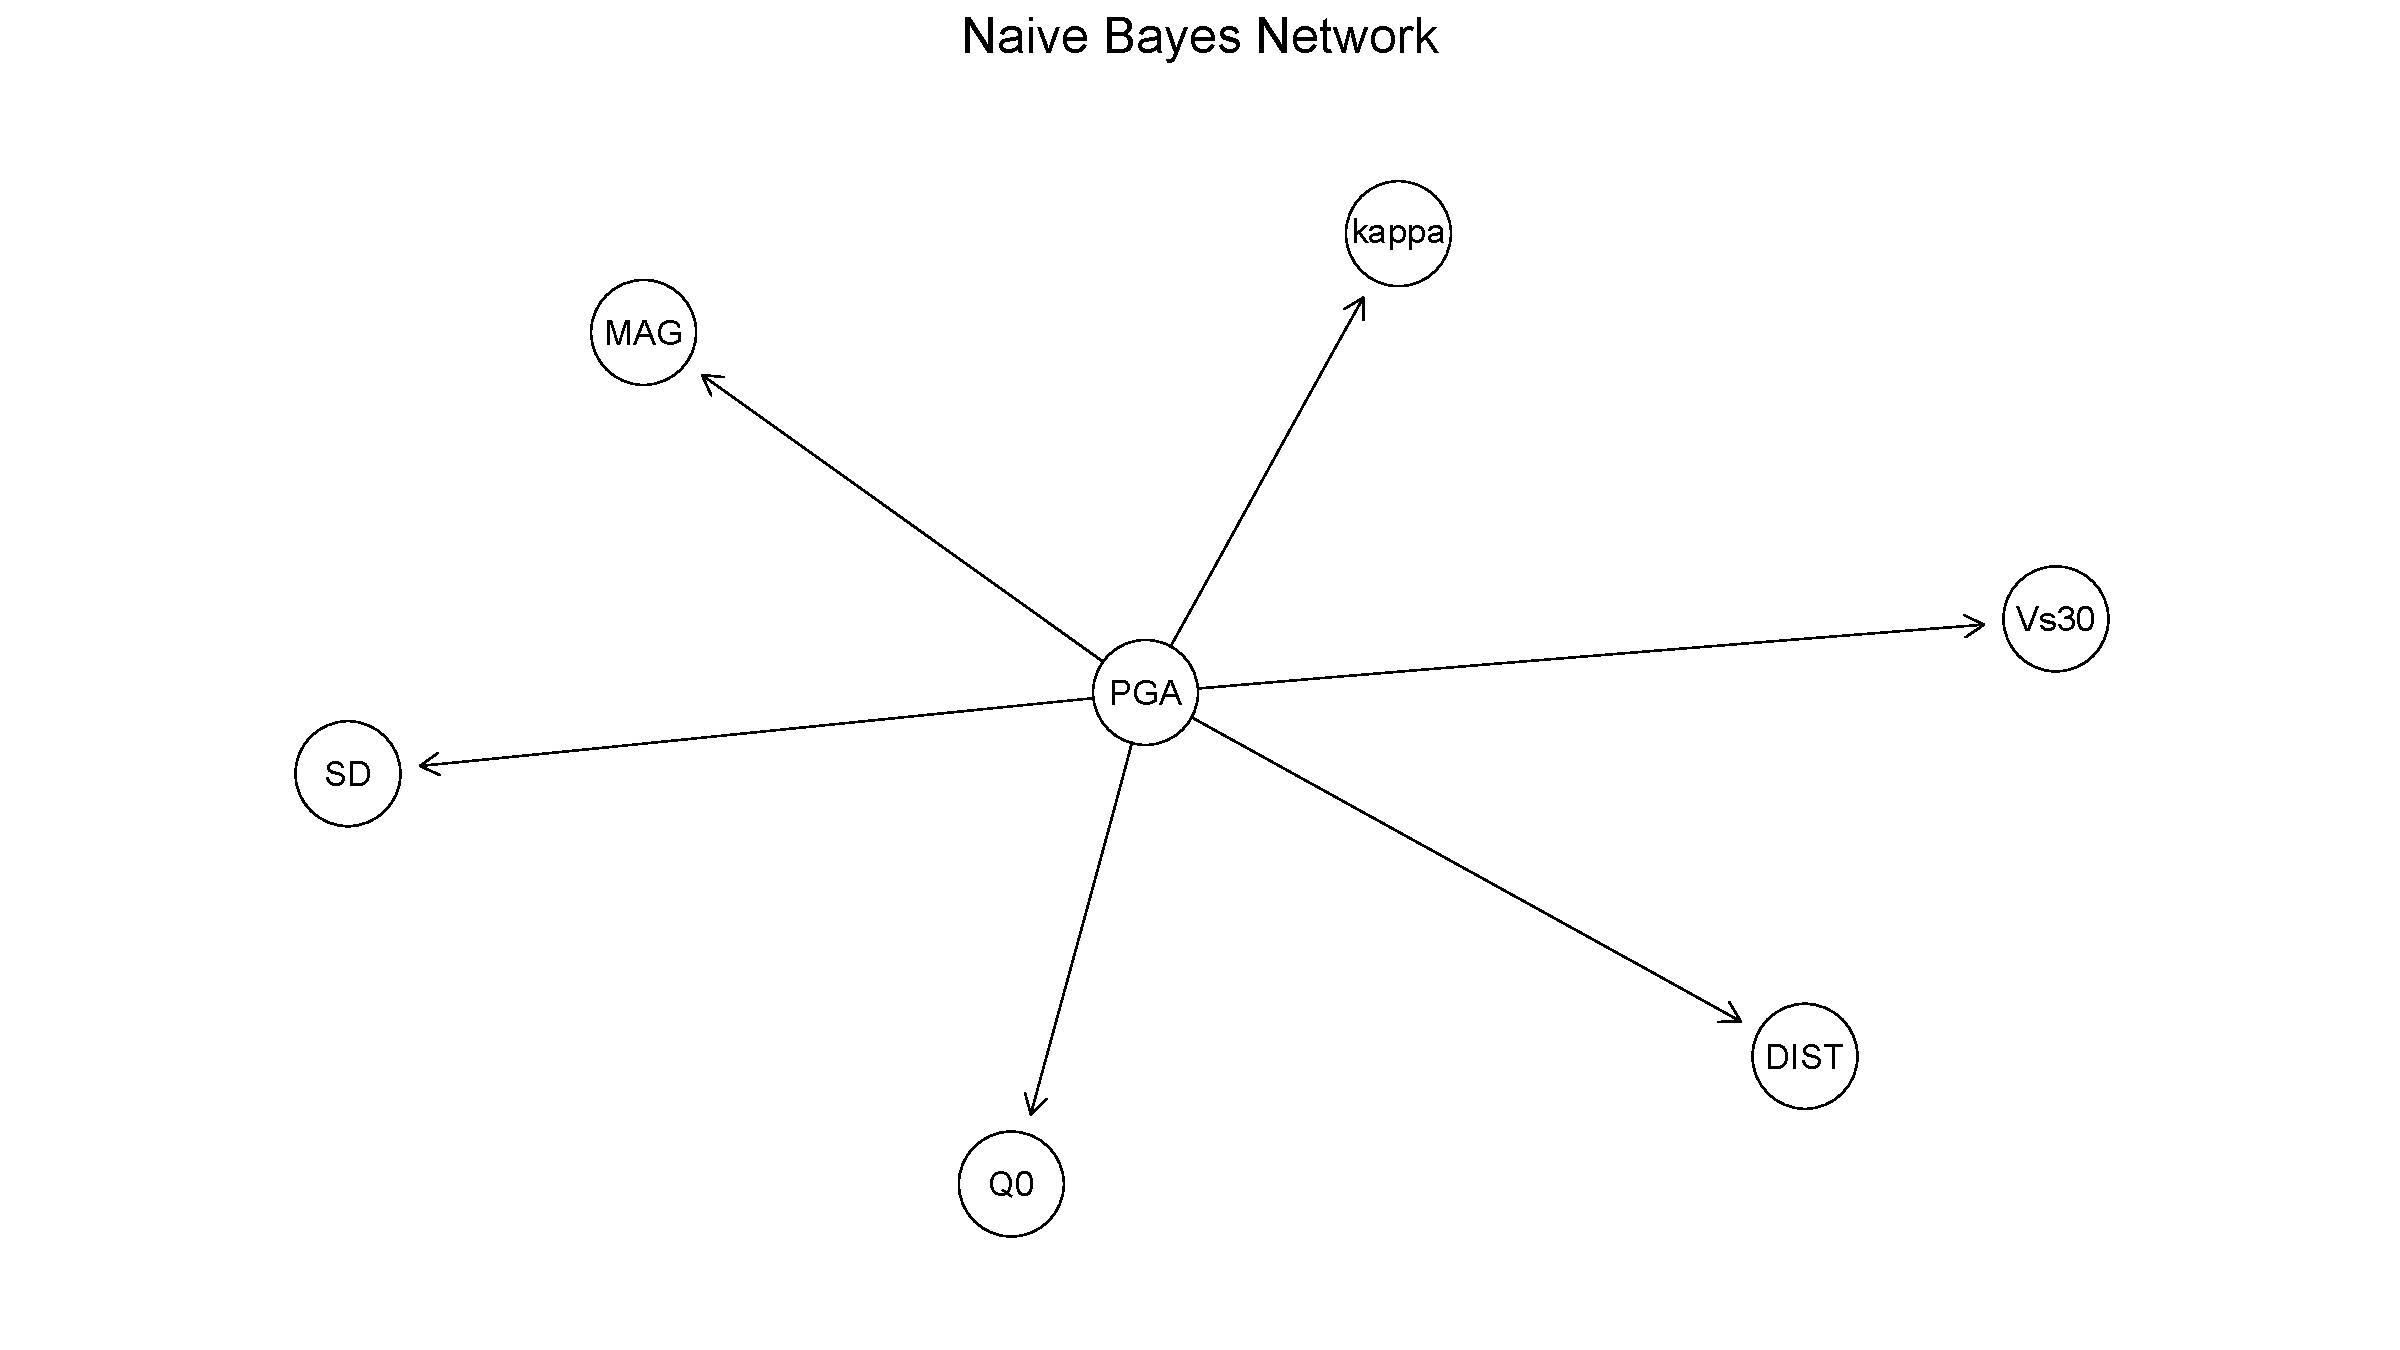
\includegraphics[scale=0.33]{Figures/naive.pdf}
		\rule{35em}{0.5pt}
	\caption[Naive Bayes Network]{A naive Bayes Network of the variables.}
	\label{fig:naive}
\end{figure}
\newpage

Another way of setting up the structure of a Bayesian Network is to rely on expert judgment to define the dependencies between the variables. This is called a causal network since one tries to capture the causal relationships in choosing the dependencies. For the case of predicting PGA from a set of explanatory variables the following causal network(Figure~\ref{fig:causal}) can be reasoned. \\

\begin{figure}[!h]
	\centering
		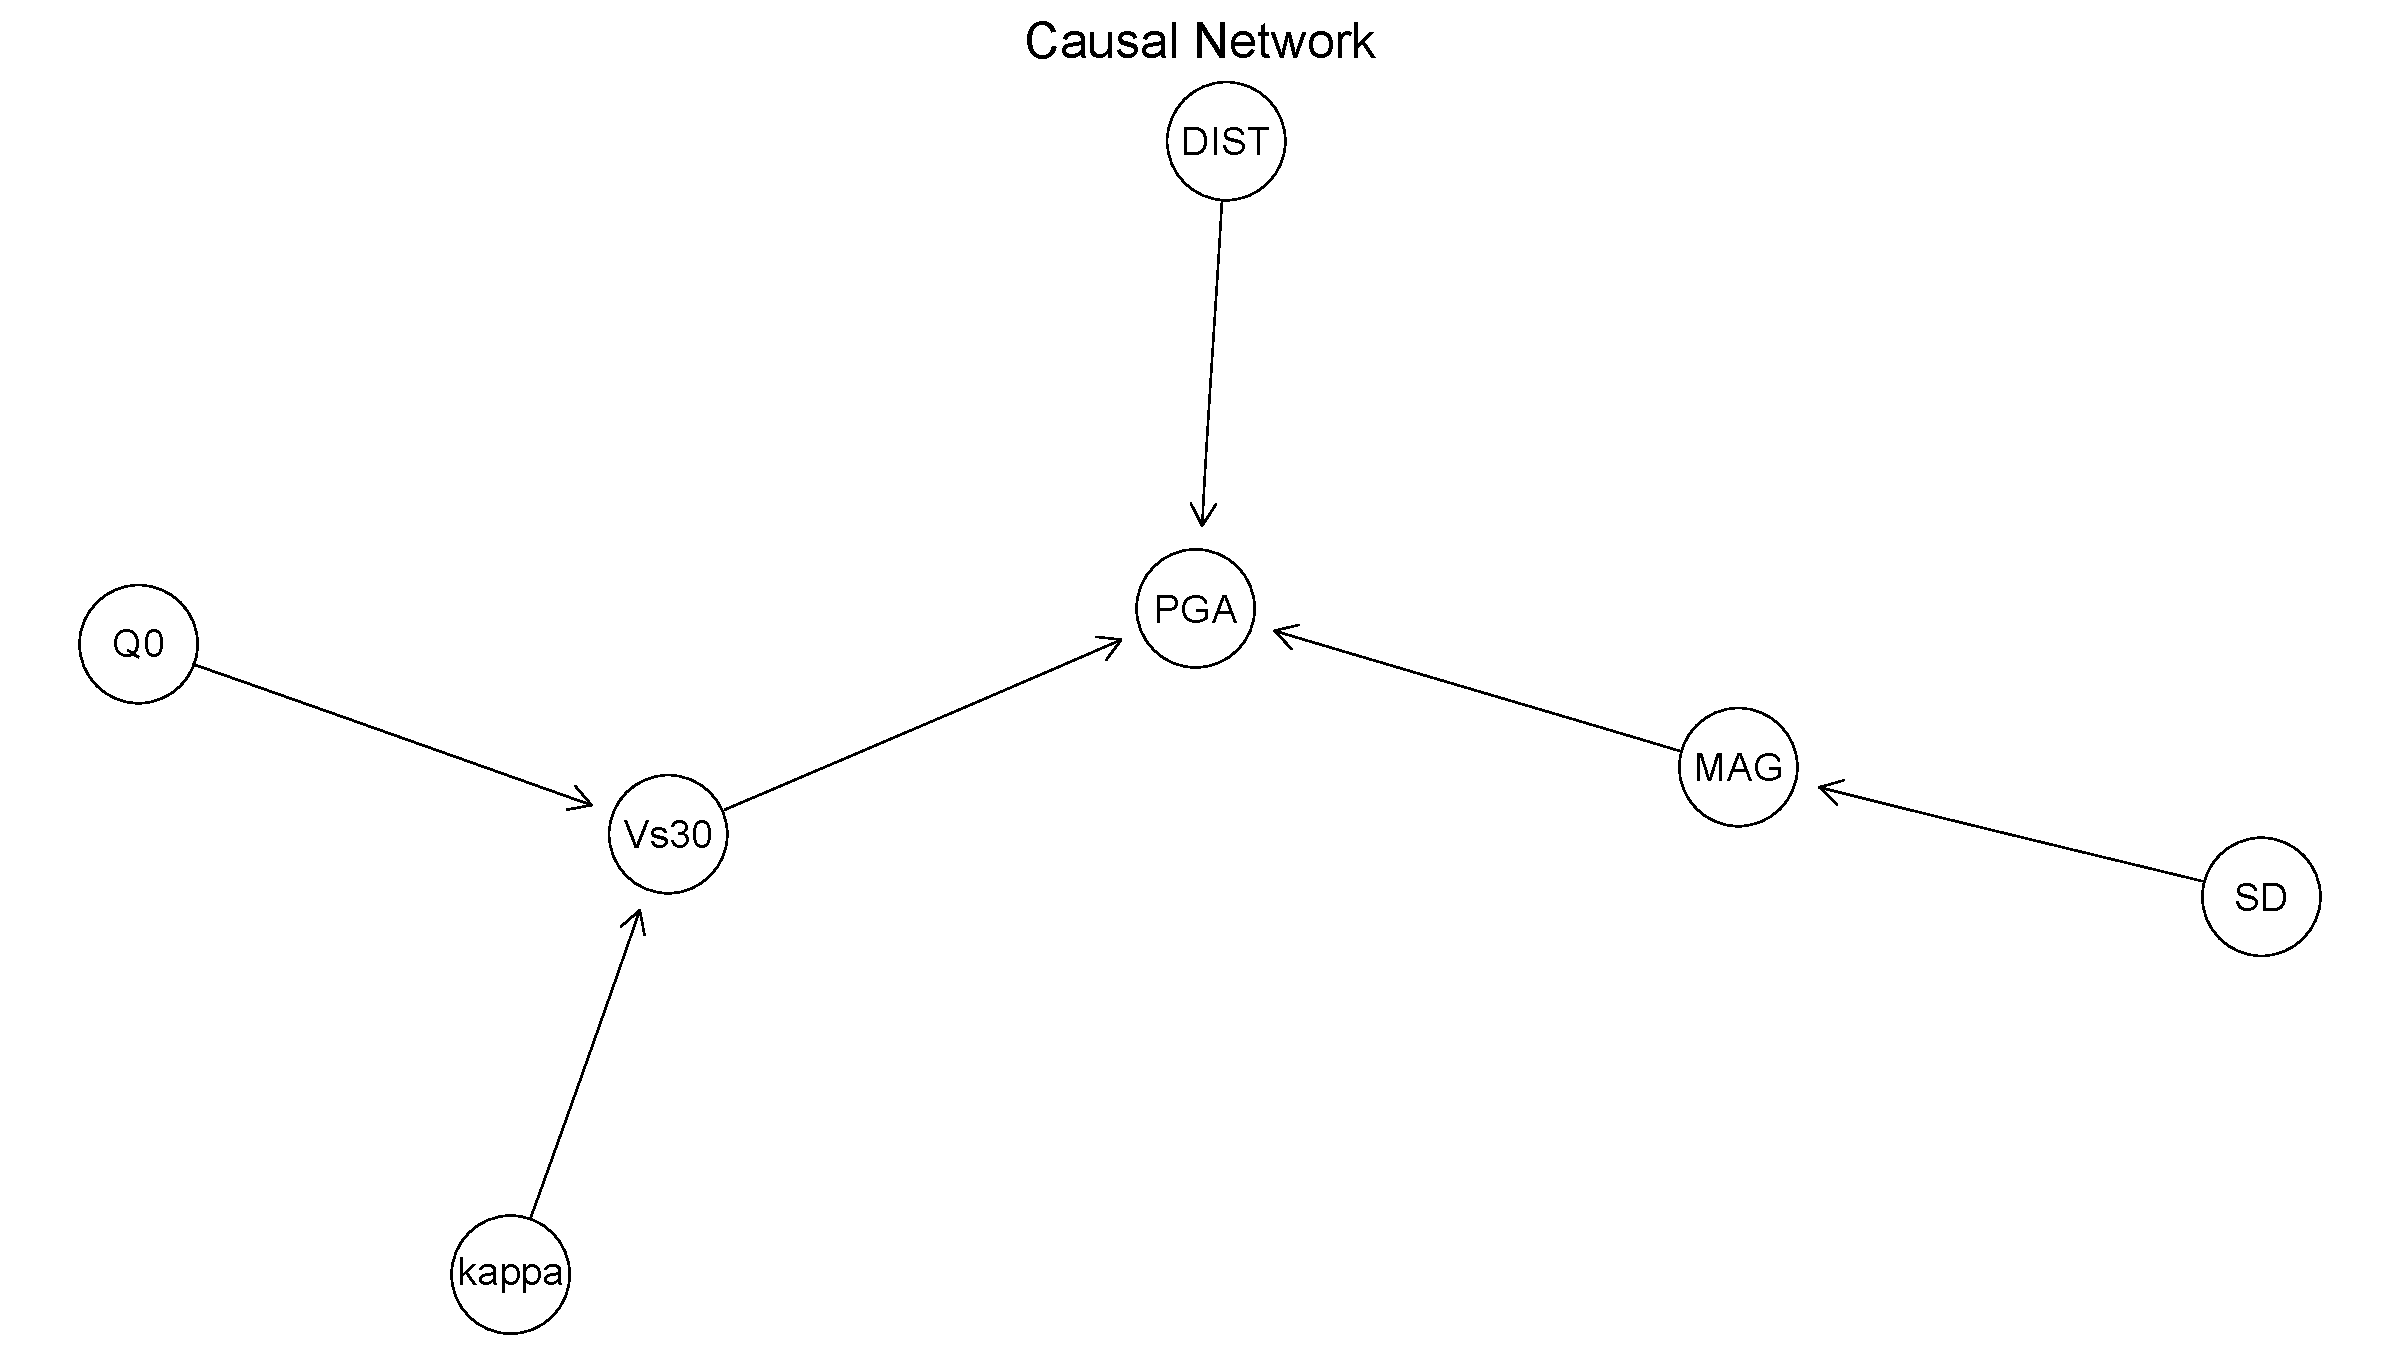
\includegraphics[scale=0.33]{Figures/causal.pdf}
		\rule{35em}{0.5pt}
	\caption[Causal Network]{A causal network representing the beliefs in dependency based on expert knowledge.}
	\label{fig:causal}
\end{figure}

One can argue that the attenuation behavior in deep layer (Q0) is independent from the one in shallow layers (kappa) because this difference reflects the varying materials and environment conditions. Nevertheless, since both are material properties, as well as the shear wave velocity in the first 30m ($V_s30$), one can imagine that their influence is mitigated by the shear wave velocity in the first 30m. The distance from the source (DIST) doesn't seem dependent on any other explanatory variable because one can imagine having the same earthquake but choosing a different location on the earth's surface. Moment magnitude (MAG) and stress drop (SD) are dependent since they both refer to the energy that is released during an earthquake. Since the moment magnitude is proportional to the ruptured area the same value can be achieved by a wide range of possible combinations in the rupture's width and length. This is the reason why it is dependent on the stress drop.\footnote{After setting up the nets and running the computations, which took almost 2 weeks, I realized that this is not the best causal network I could design through my knowlegde of the earthquake process. Q0 and kappa are attenuation parameters and only influence the amplitude of the seismic waves. It is questionable how this can have an influence on the seismic wave velocity. There also might be a dependency between the distance and the magnitude since larger earthquakes appear in greater depths and the distance employed in the Boore model is hypocentral distance and not epicentral. So this is more an example of a poorly designed causal net.}\\
Another way to set up causal networks is to consult literatur about the topic. In the case of Bayesian Networks for ground motion prediction sources could be \cite{kuehn2010} or \cite{Vogel2014}.\\

A third way of defining the structure of a Bayesian network is to learn it from the data itself. Often, not all dependencies between the variables are known and human domain knowledge can also be misleading. So it is a natural extension to ask whether there are principled ways in the framework of Bayesian networks to let also the structure come from the data. This can be done by extending the Bayesian paradigm so that the structure of a network becomes a random variable, too. Now the task is to jointly estimate the parameters and the structure from the data. In the scope of this paper the constraint-based Grow-Shrink algorithm~\citep{margaritis2003} and the score-based hill-climber are explored.\\
Constraint-based algorithms perform independence tests between the random variables and then set up a network according to the found independencies. The task is one of finding the best minimal I-map. An I-map or independence map is a graph whose independence statements hold for the probability distribution one tries to model. In the case where the graph captures all independence statements this is a perfect I-map. A minimal I-map is graph that is rendered not an I-map anymore by the removal of one edge. This is an important definition because the complete graph over a set of random variables is also an I-map but does not reveal any independencies and therefore carries parameters that are redundant. In practice one does not find one single best minimal I-map but a class of graphs that carry the same independence statements and are therefore called I-equivalent~\citep{koller2009}. 
The Grow-Shrink algorithm tries to construct the structure of a network by finding the Markov Blankets of the variables. A Markov Blanket of one variable is a set of variables that renders that variable to be d-separated from all other variables. That means that knowing the state of any variable that is not in the Markov Blanket has no effect on knowing the state of the variable in interest. One could say that the Markov Blanket "shields" a variable from the influence of all other variables. Graphically it is the set of parents, children and parents of the children of the variable in interest~\citep{koller2009}. In the Growing phase of the Grow-Shrink algorithm independence tests between variables are performed which are the basis to decide whether a variable should be included in the Markov blanket. These test occur given the state of the Markov Blanket. Depending on the initial ordering of the variables this can lead to include redundant variables in the Markov Blanket which are subsequently removed by the independence test of the Shrinking phase~\citep{margaritis2003}. For learning the structure of a Bayesian network according to the Grow-Shrink algorithm the mutual information (Equation~\ref{eqn:mutual}) is used as an independence test.

\begin{equation}
I(X;Y) = \sum_{y \in Y} \sum_{x \in X} 
                 p(x,y) \log{ \left(\frac{p(x,y)}{p(x)\,p(y)}
                              \right) }, \,\! 
\label{eqn:mutual}
\end{equation}

It estimates the dependence between two variables by comparing the joint distribution to the product of the marginal distributions, since in the case of independence the joint distribution factorizes to the product of the marginal distributions. From a Venn-diagram point of view it calculates the area shared by two variables relative to the total area of the variables.\\
The learned network is visualized in Fig.\ref{fig:gs}. There are no direct dependencies between the explanatory variables. Even more the variable $V_s30$ is completely ignored. By comparing this result to work of~\citep{Vogel2014}which uses a similar data set\footnote{ ;)} one can find that this seems to be a consistent result when learning the structure of a Bayesian network for ground motion prediction from data. One reason might be that $V_s30$ is merely a proxy in quantifying the capability of the soil to amplify the amplitudes of seismic waves.\\

\begin{figure}[htbp]
	\centering
		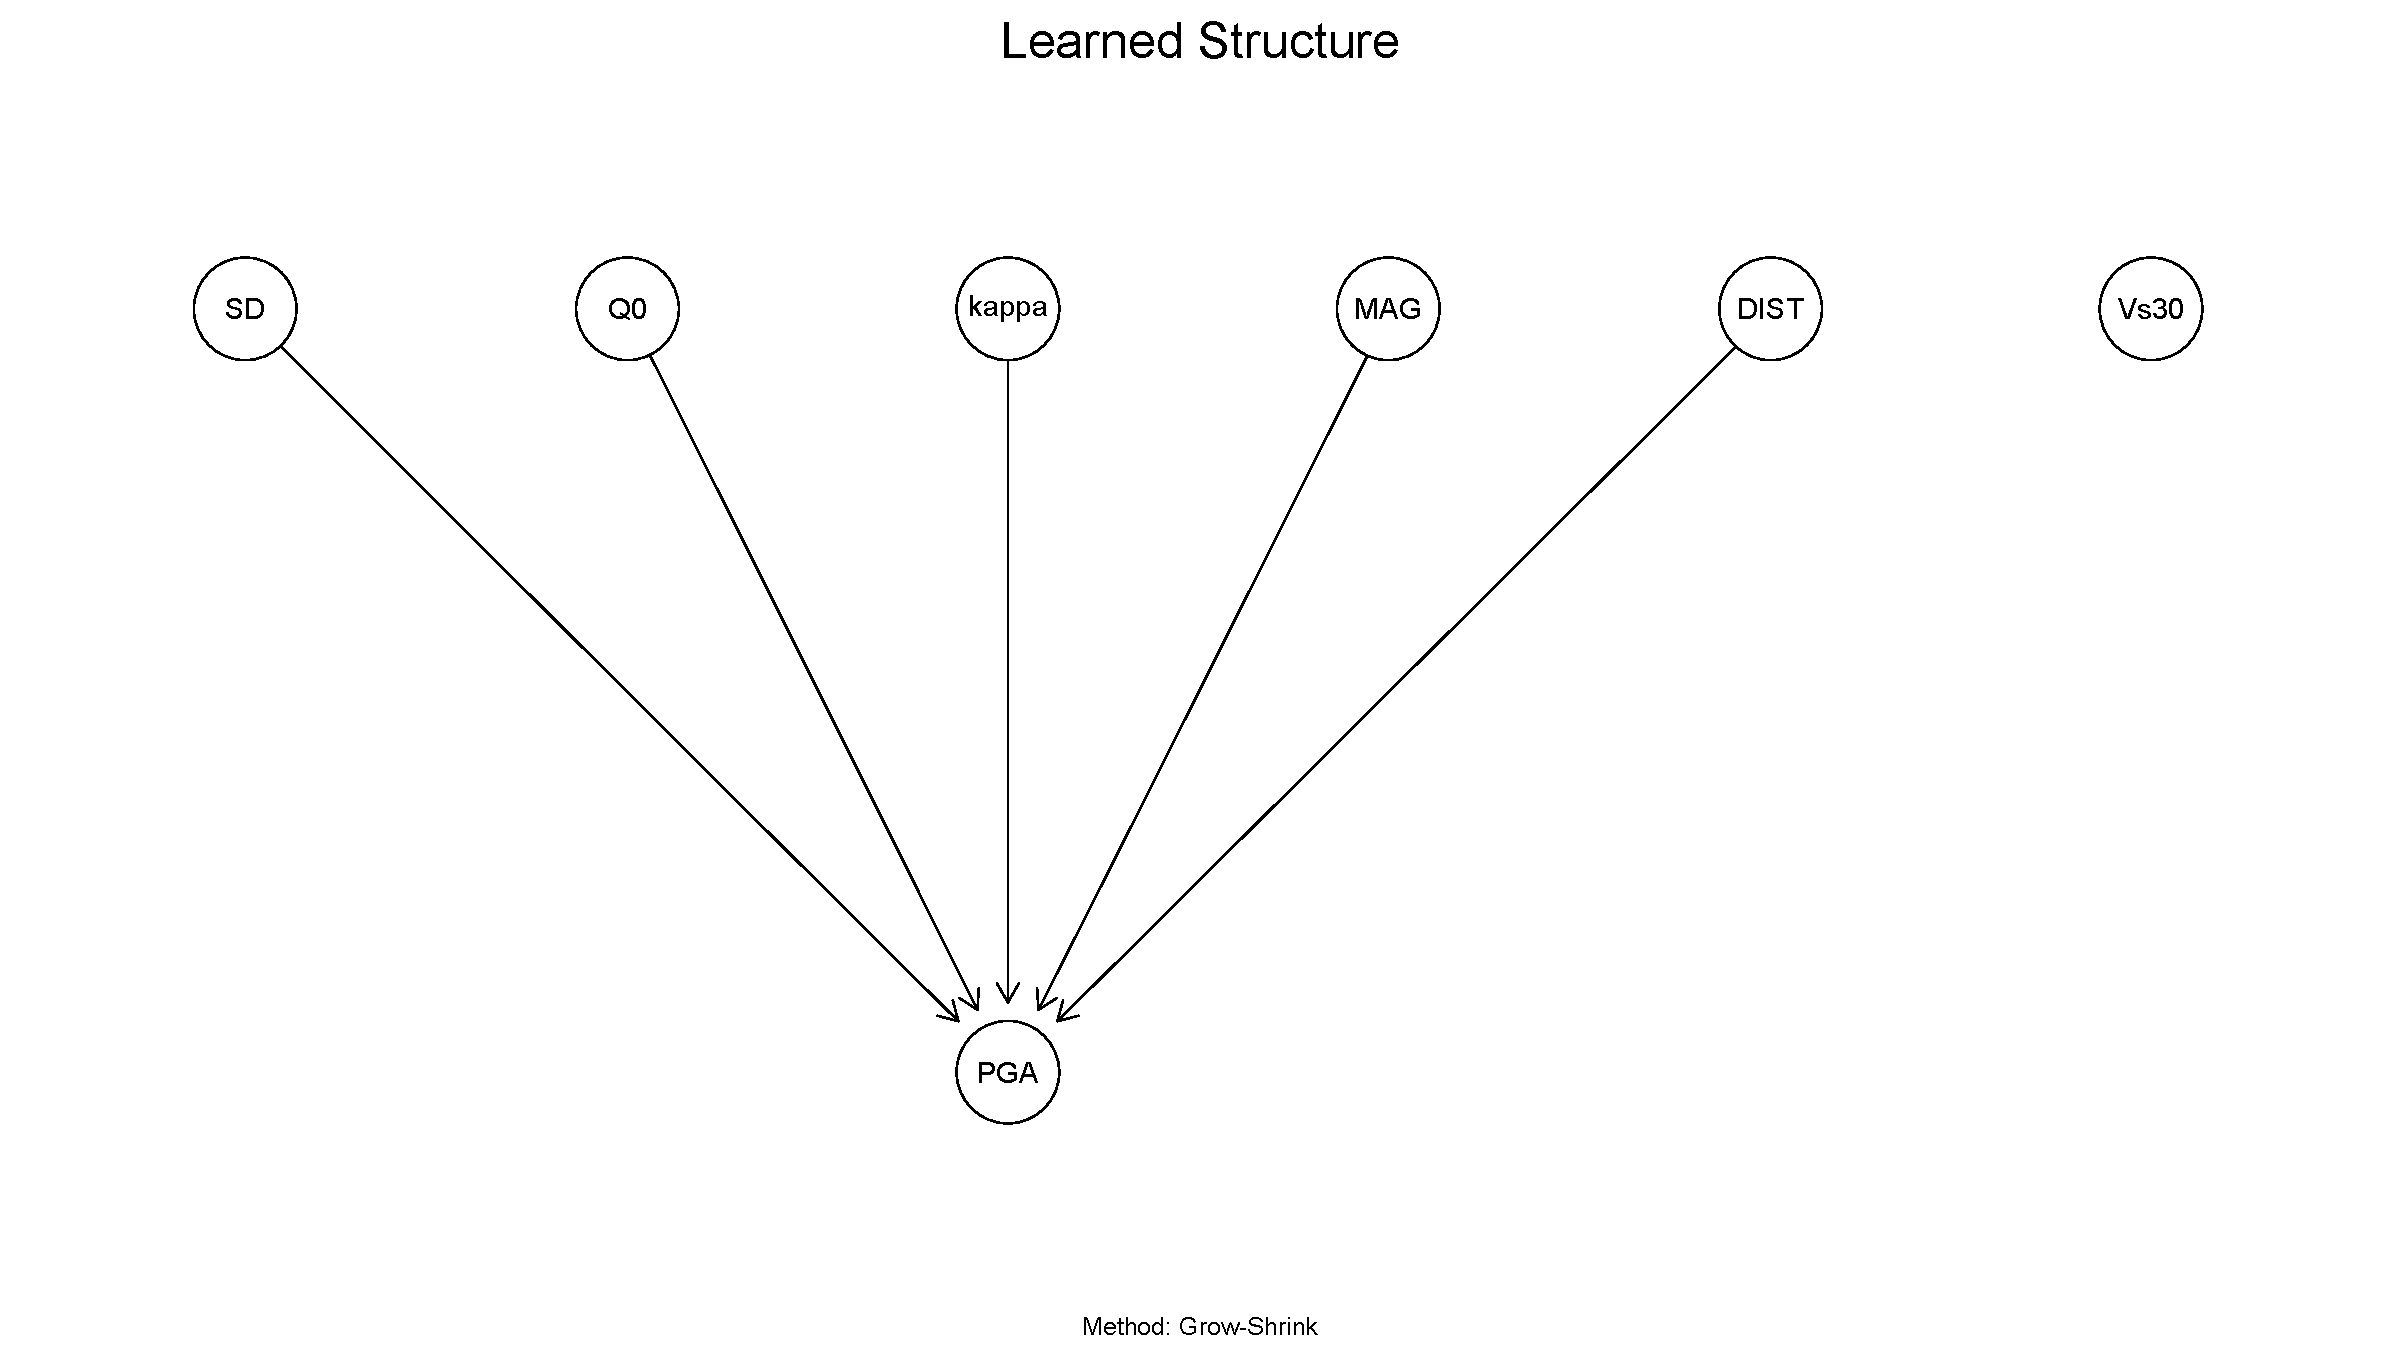
\includegraphics[scale=0.33]{Figures/gs_one.pdf}
		\rule{35em}{0.5pt}
	\caption[Contraint-based Grow-Shrink Network]{Bayesian Network constructed by the Grow-Shrink algorithm.}
	\label{fig:gs}
\end{figure}

Score-based algorithms view the problem of finding the structure of a Bayesian network from an optimization point of view. In contrast to the constraint-based algorithms, score-based ones do not try to construct the structure from information about single dependencies between variables, but take the network as a whole, compute a score that measures whether the current structure could have generated the data and try to find the network that maximizes that score. Consequently, score-based algorithm pose a search problem in the space of possible network structures. Depending on the number of variables and the underlying probability distribution in most cases this is a NP-hard problem and requires some approximation techniques~\citep{koller2009}.\\
A Hill-climber can be thought of as the opposite of gradient descent since it tries to maximize a predefined score in contrast to minimizing an error term. For the construction of a Bayesian network using the hill-climber algorithm a score consisting of the maximized likelihood L (Equation \ref{eqn:likelihood}) that gives the probability of the data being generated by the graph G and the parameters $\theta$ and the Bayesian Information Criterion (BIC) (Equation~\ref{eqn:BIC}~\citep{schwarz}) as a regularization term consisting of the number of free parameters $k$ and the size of the data $n$ is used.

\begin{equation}
L = \operatorname*{arg\,max}_\theta P(x\mid \theta, G)
\label{eqn:likelihood}
\end{equation}

\begin{equation}
BIC = -2*ln L + k* ln(n)
\label{eqn:BIC}
\end{equation}


\begin{figure}[htbp]%
	\centering
		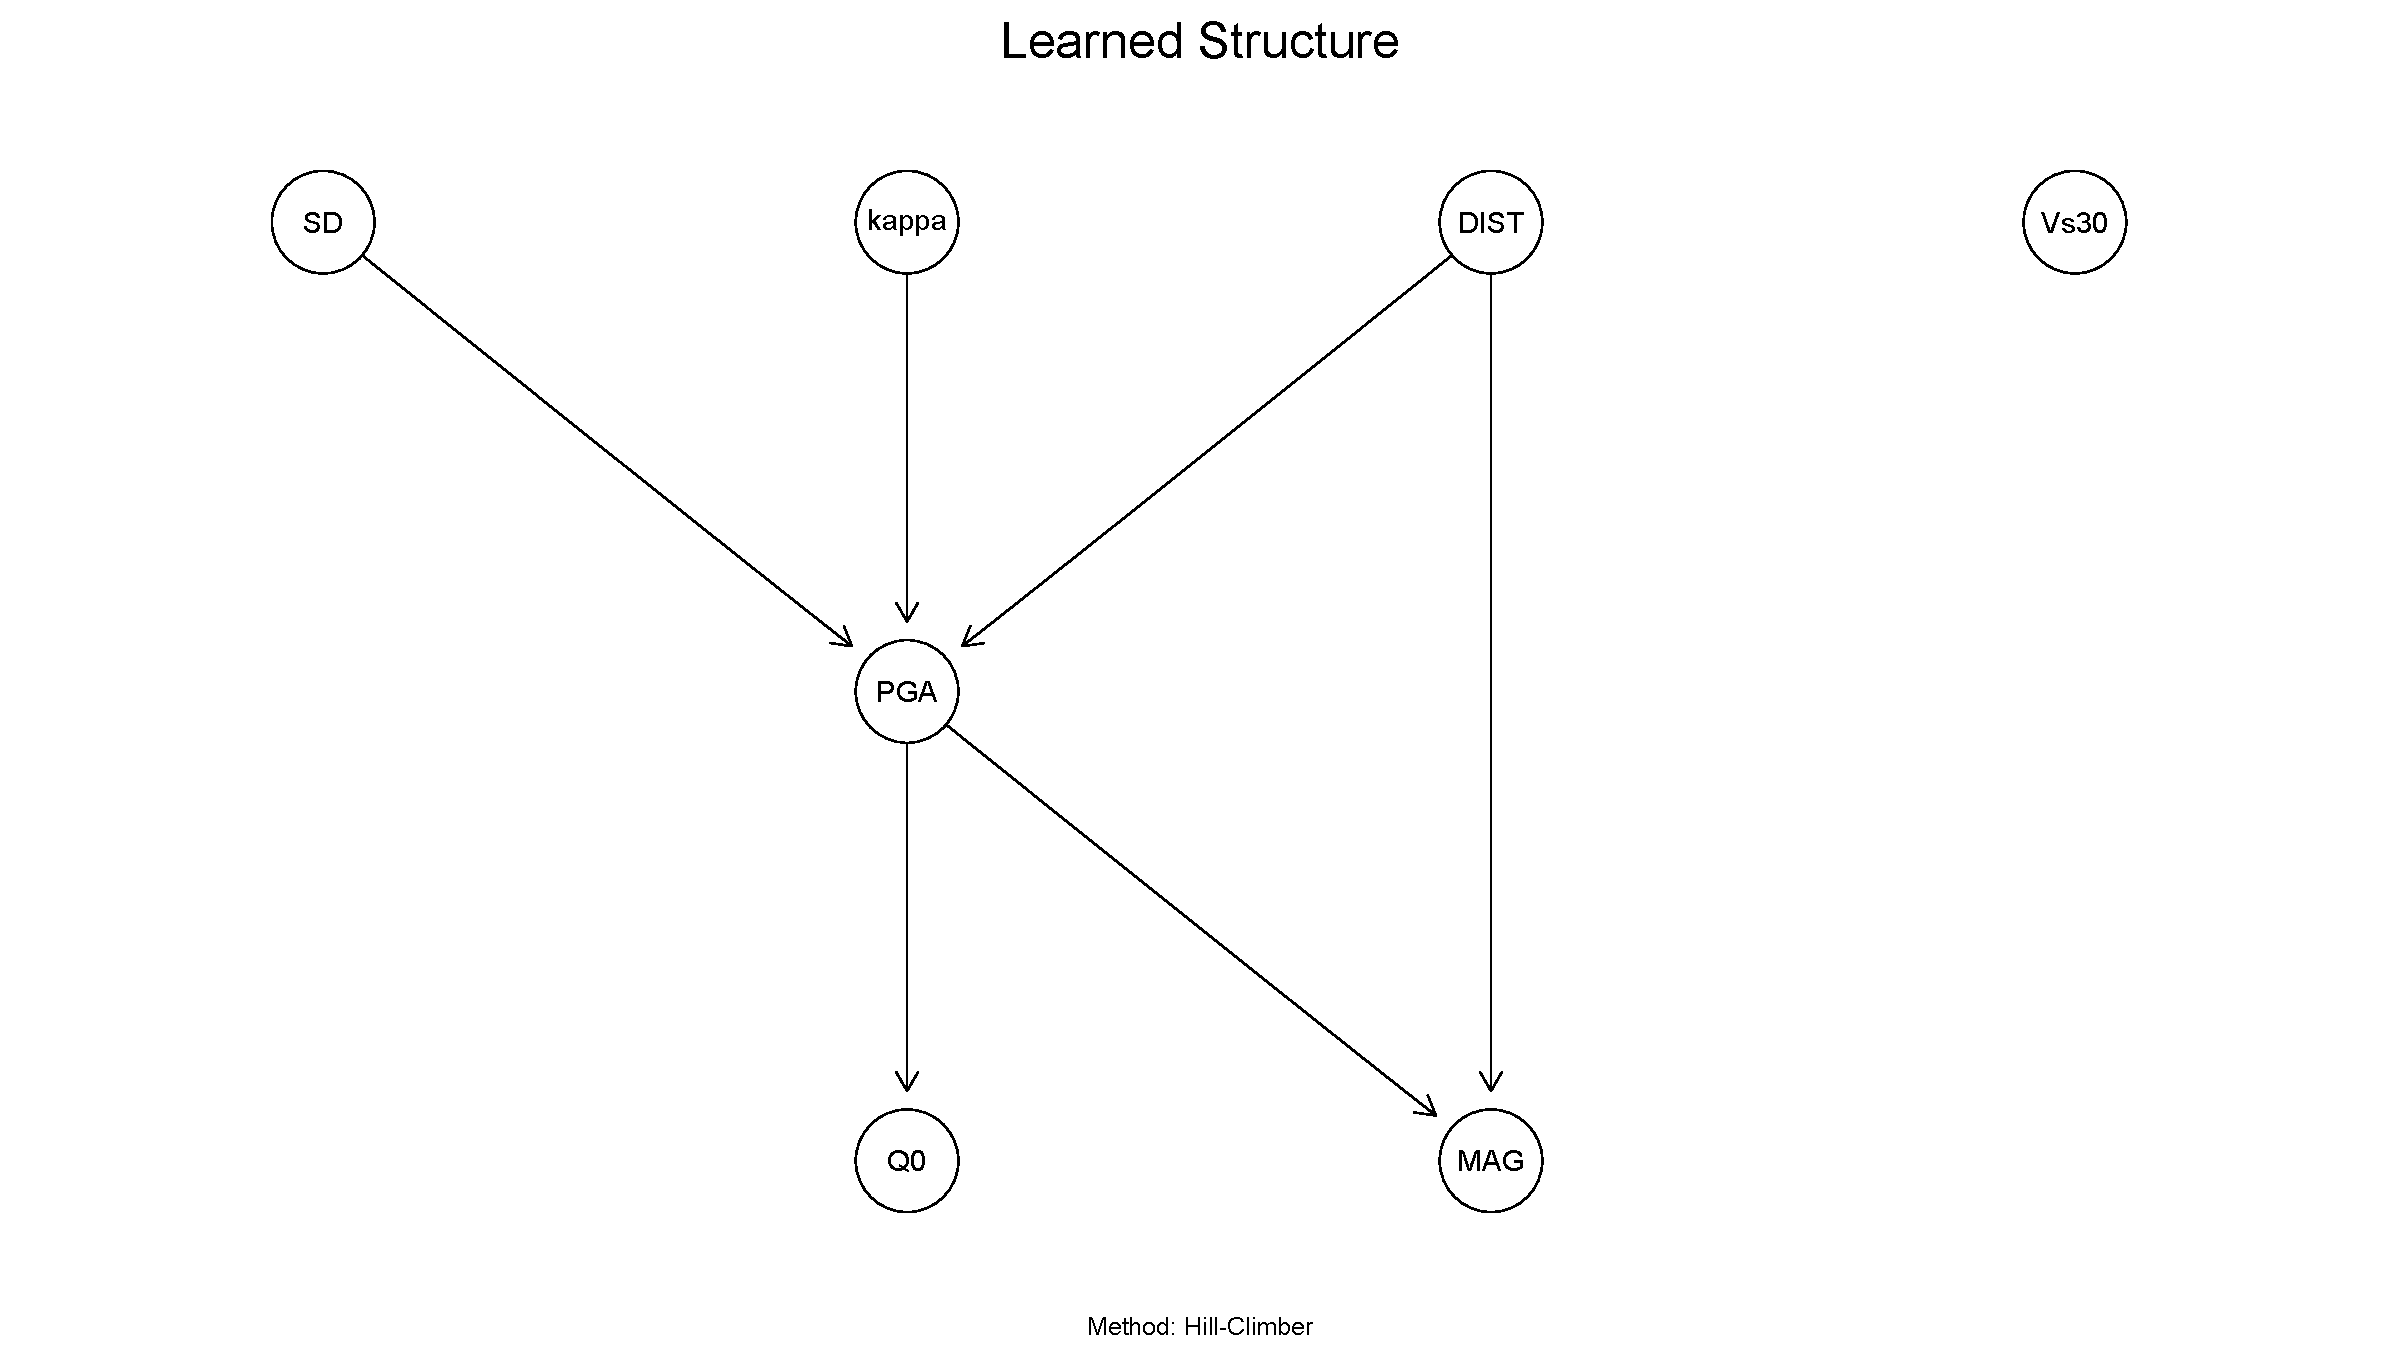
\includegraphics[scale=0.33]{Figures/hc_one.pdf}
		\rule{35em}{0.5pt}
	\caption[Score-based Hill-Climber Network]{hc}
	\label{fig:hc}
\end{figure}

The learned structure networks look pretty similar. Compare to \citep{Vogel2014} because they are from similar data. Actually a series of networks was learned: \ref{AppendixA1} \ref{AppendixA2}

%----------------------------------------------------------------------------------------

\section{Parameter Learning}
\begin{table}[h]
\begin{tabular}{l|c c c c c c c c c  }
\hline
SD:&         0&  0.8792&   5.438&  14.92&       58&   500&      &      & \\
Q0:&         0&     330&    5000&       &         &      &      &      & \\
$\kappa_0$:& 0& 0.01053&  0.0345&    0.1&         &      &      &      & \\
VS30:&     600&  1704.5&    2800&       &         &      &      &      & \\
M:&          5&   6.271&     7.5&       &         &      &      &      & \\
R:&          1&    4.38& 15.4885&  55.84&      200&      &      &      & \\
log PGA:& -Inf&  -5.135&  -3.722& -2.627& -1.20742& 0.145& 1.657& 3.175& Inf\\
\end{tabular}
\caption[Discretization of the Variables]{Discretization of the Variables.}
\label{tab:2}
\end{table}


Since the analytic form of the stochastic ground motion model by~\cite{boore2003} is very complex the data is divided into intervals and the BNS are discrete.


bayesian parameter estimation
%----------------------------------------------------------------------------------------

